%*******************************************************************************
%*********************************** First Chapter *****************************
%*******************************************************************************

\chapter{Introduction}  %Title of the First Chapter

\ifpdf
\graphicspath{{Chapter1/Figs/Raster/}{Chapter1/Figs/PDF/}{Chapter1/Figs/}}
\else
\graphicspath{{Chapter1/Figs/Vector/}{Chapter1/Figs/}}
\fi


%********************************** %First Section  **************************************
\section{Motivation}
With the advancement in medical imaging, computer aided diagnostic systems have become a vital part of today's medical diagnosis\cite{doi2007computer}. CAD systems have become a part of routine clinical work and are being used extensively for diseases diagnosis.A myriad of different medical imaging systems,like X-Ray, Magnetic Resonance Imaging (MRI), Computed Tomography Scans etc, are used for diagnosis. The output of such systems are multi dimensional digital images, interpretation of which require sophisticated digital image processing methods. Automated medical diagnosis systems can aid in easy and faster interpretation of these images.\\	

Digital fundus imaging in ophthalmology is a vital component in diagnosis of various pathologies like Diabetic Retinopathy(DR),glaucoma and age related macular degeneration(AMD), . Retinal vessel segmentation forms an important part of diagnosis of such pathologies. Changes in the retinal vascualture is precursor to many diseases such as diabetes,hypertension and stroke. Morphological properties such as diameter, length, branching angle, of the retinal vessel forms an important component in diagnosis and evaluation of ophthalmologic diseases such as diabetic retinopathy \cite{sinthanayothin2002automated} and hypertension. For example, vessel diameter measurement can be an aid in diagnosis of hypertension\cite{calvo2011automatic}.\\

Vessel segmentation in itself is a challenging and a tedious task which may take a couple of hours when performed manually. Problems like low contrast between vessel and background, noise in the image and variability in the width, brightness and shape alongwith the presence of exudates,lesions, hemorrhage spots and other pathological effects make the task much more difficult. Figure \ref{fig:fundusdiseased} shows a fundus image of a diseased eye.\\

\begin{figure}
	\centering	
	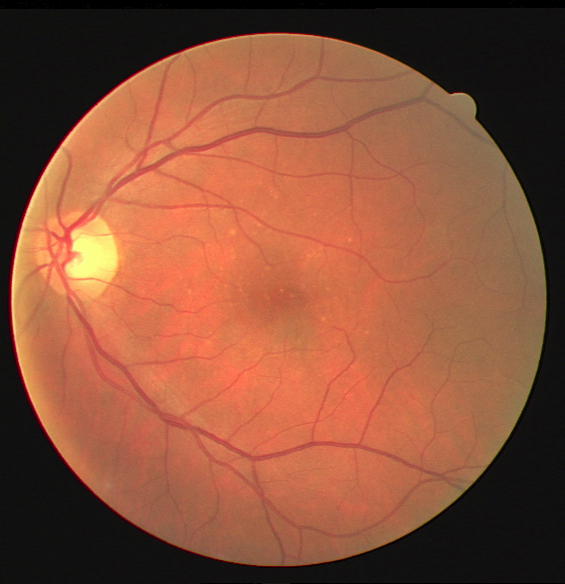
\includegraphics[width=0.5\textwidth]{fundusimage.png}
	\caption{A diseased fundus image}
	\label{fig:fundusdiseased}		
\end{figure}	

Developing an automated retinal vessel segmentation is a first step towards developing a full fledged CAD system for diagnosis of ophthalmology pathologies. There have been a lot of work in literature on automatic retinal segmentation, including based on matched filtering\cite{zana2001segmentation,hoover2000locating,al2007improved}, tracking methods[\cite{mendonca2006segmentation,chutatape1998retinal}], morphological methods\cite{leandro2001blood,walter2001segmentation}, and learning based methods\cite{sopharak2010machine,fuller2007segmentation,niemeijer2007automated}. Some of the simplest approaches to segmentation use adaptive thresholding to segment out the blood vessels\cite{jiang2003adaptive}. Another simple approach is to use edge detection techniques like canny edge detector for vessel segmentation\cite{chrastek2002optic}.\\

Some of the more sophisticated models use learning based algorithms which learn on a set of given image segmentations. Many of these models, learn local features at a pixel location and train a pixel based classifier.\citep{nguyen2011effective} present the limitations in some of the state-of-art methods and presents a multi scale line detection based method for blood vessel segmentation.Issues, like poor segmentation at bifurcation and crossover regions, merging of close vessels and poor segmentation of small vessels limit the application of vasculature based medical diagnosis.For example, merging of two nearby vessels can lead to vessel being considered as one wide vessel, thereby affecting the width measurements of the vessel. These limitations may contribute to inaccuracies in vascular network analysis and subsequently in characterization of diseases. \\

\begin{figure}
	\centering	
	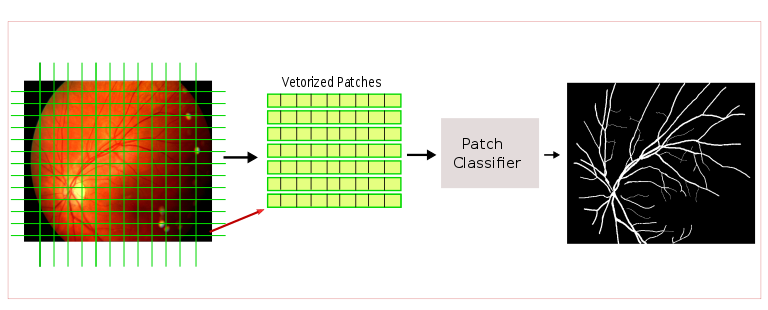
\includegraphics[width=0.8\textwidth]{model.png}
	\caption{Architecture for automated segmentation of retinal vessels.}
	\label{fig:basicmodel}		
\end{figure}
Supervised learning methods, in general are limited by the amount of training data.Also most of them are restricted to the type of training data and do not generalize on the task at hand. In our thesis, we propose two supervised learning models for accurate vessel segmentation. Our method is a patch-based framework and learns the local structure of the vessel at patch level. An illustrative architecture of our framework is shown in figure \ref{fig:basicmodel}, exploits the presence of common structures in a typical vasculature tree. Unlike most of the supervised learning methods which make a prediction at pixel level, classifying each pixel as vessel or background, our model predicts the local structure around each pixel at patch level.

\section{Outline of thesis}
The thesis is organized as follow,
\begin{itemize}
	\item Chapter 2 provides some background knowledge on machine learning and used algorithms. It is followed by a brief overview on existing work on blood vessel segmentation.Finally, we explain in detail some of the methods by which our work is inspired.
	\item Chapter 3 starts by defining our patch-based framework for vessel segmentation. We then explain our models based on cluster learning and dictionary learning.
	\item Chapter 4 presents the evaluations and experimental results of our methods applied to three datasets. We present the effect of different setting on the performance. We also compare our evaluations with some of the work in the literature.
	\item Chapter 5, finally gives our concluding remarks and sets the tone for future work that can be carried on this approach. 
\end{itemize}